%This is a template file for use of iopjournal.cls

\documentclass{iopjournal}
\usepackage{subcaption} 
\usepackage{placeins} 
\usepackage{amsmath}
\usepackage{booktabs}
\usepackage{ragged2e}
\usepackage{siunitx}
\usepackage{makecell}


% Options
% 	[anonymous]	Provides output without author names, affiliations or acknowledgments to facilitate double-anonymous peer-review

\begin{document}

\articletype{Paper} %	 e.g. Paper, Letter, Topical Review...

\title{Title}

\author{Lukas Wolff$^1$, Álvaro Paul$^1$, Patricio A. Moreno-Casas$^{1,*}$}

\affil{$^1$Facultad de Ingeniería y Ciencias Aplicadas, Universidad de los Andes, Chile}\\
\affil{$^2$Carrera de Ingeniería Civil, Universidad Andres Bello, Chile}

%\affil{$^*$Author to whom any correspondence should be addressed.}
\email{patriciomoreno@miuandes.cl}

\keywords{}

\begin{abstract}
T
\end{abstract}


\section{Introduction}


\section{Methodology}

\subsection{Experimental Setup}

\subsubsection{Multi-camera configuration}

\begin{figure}[htb]
    \centering
    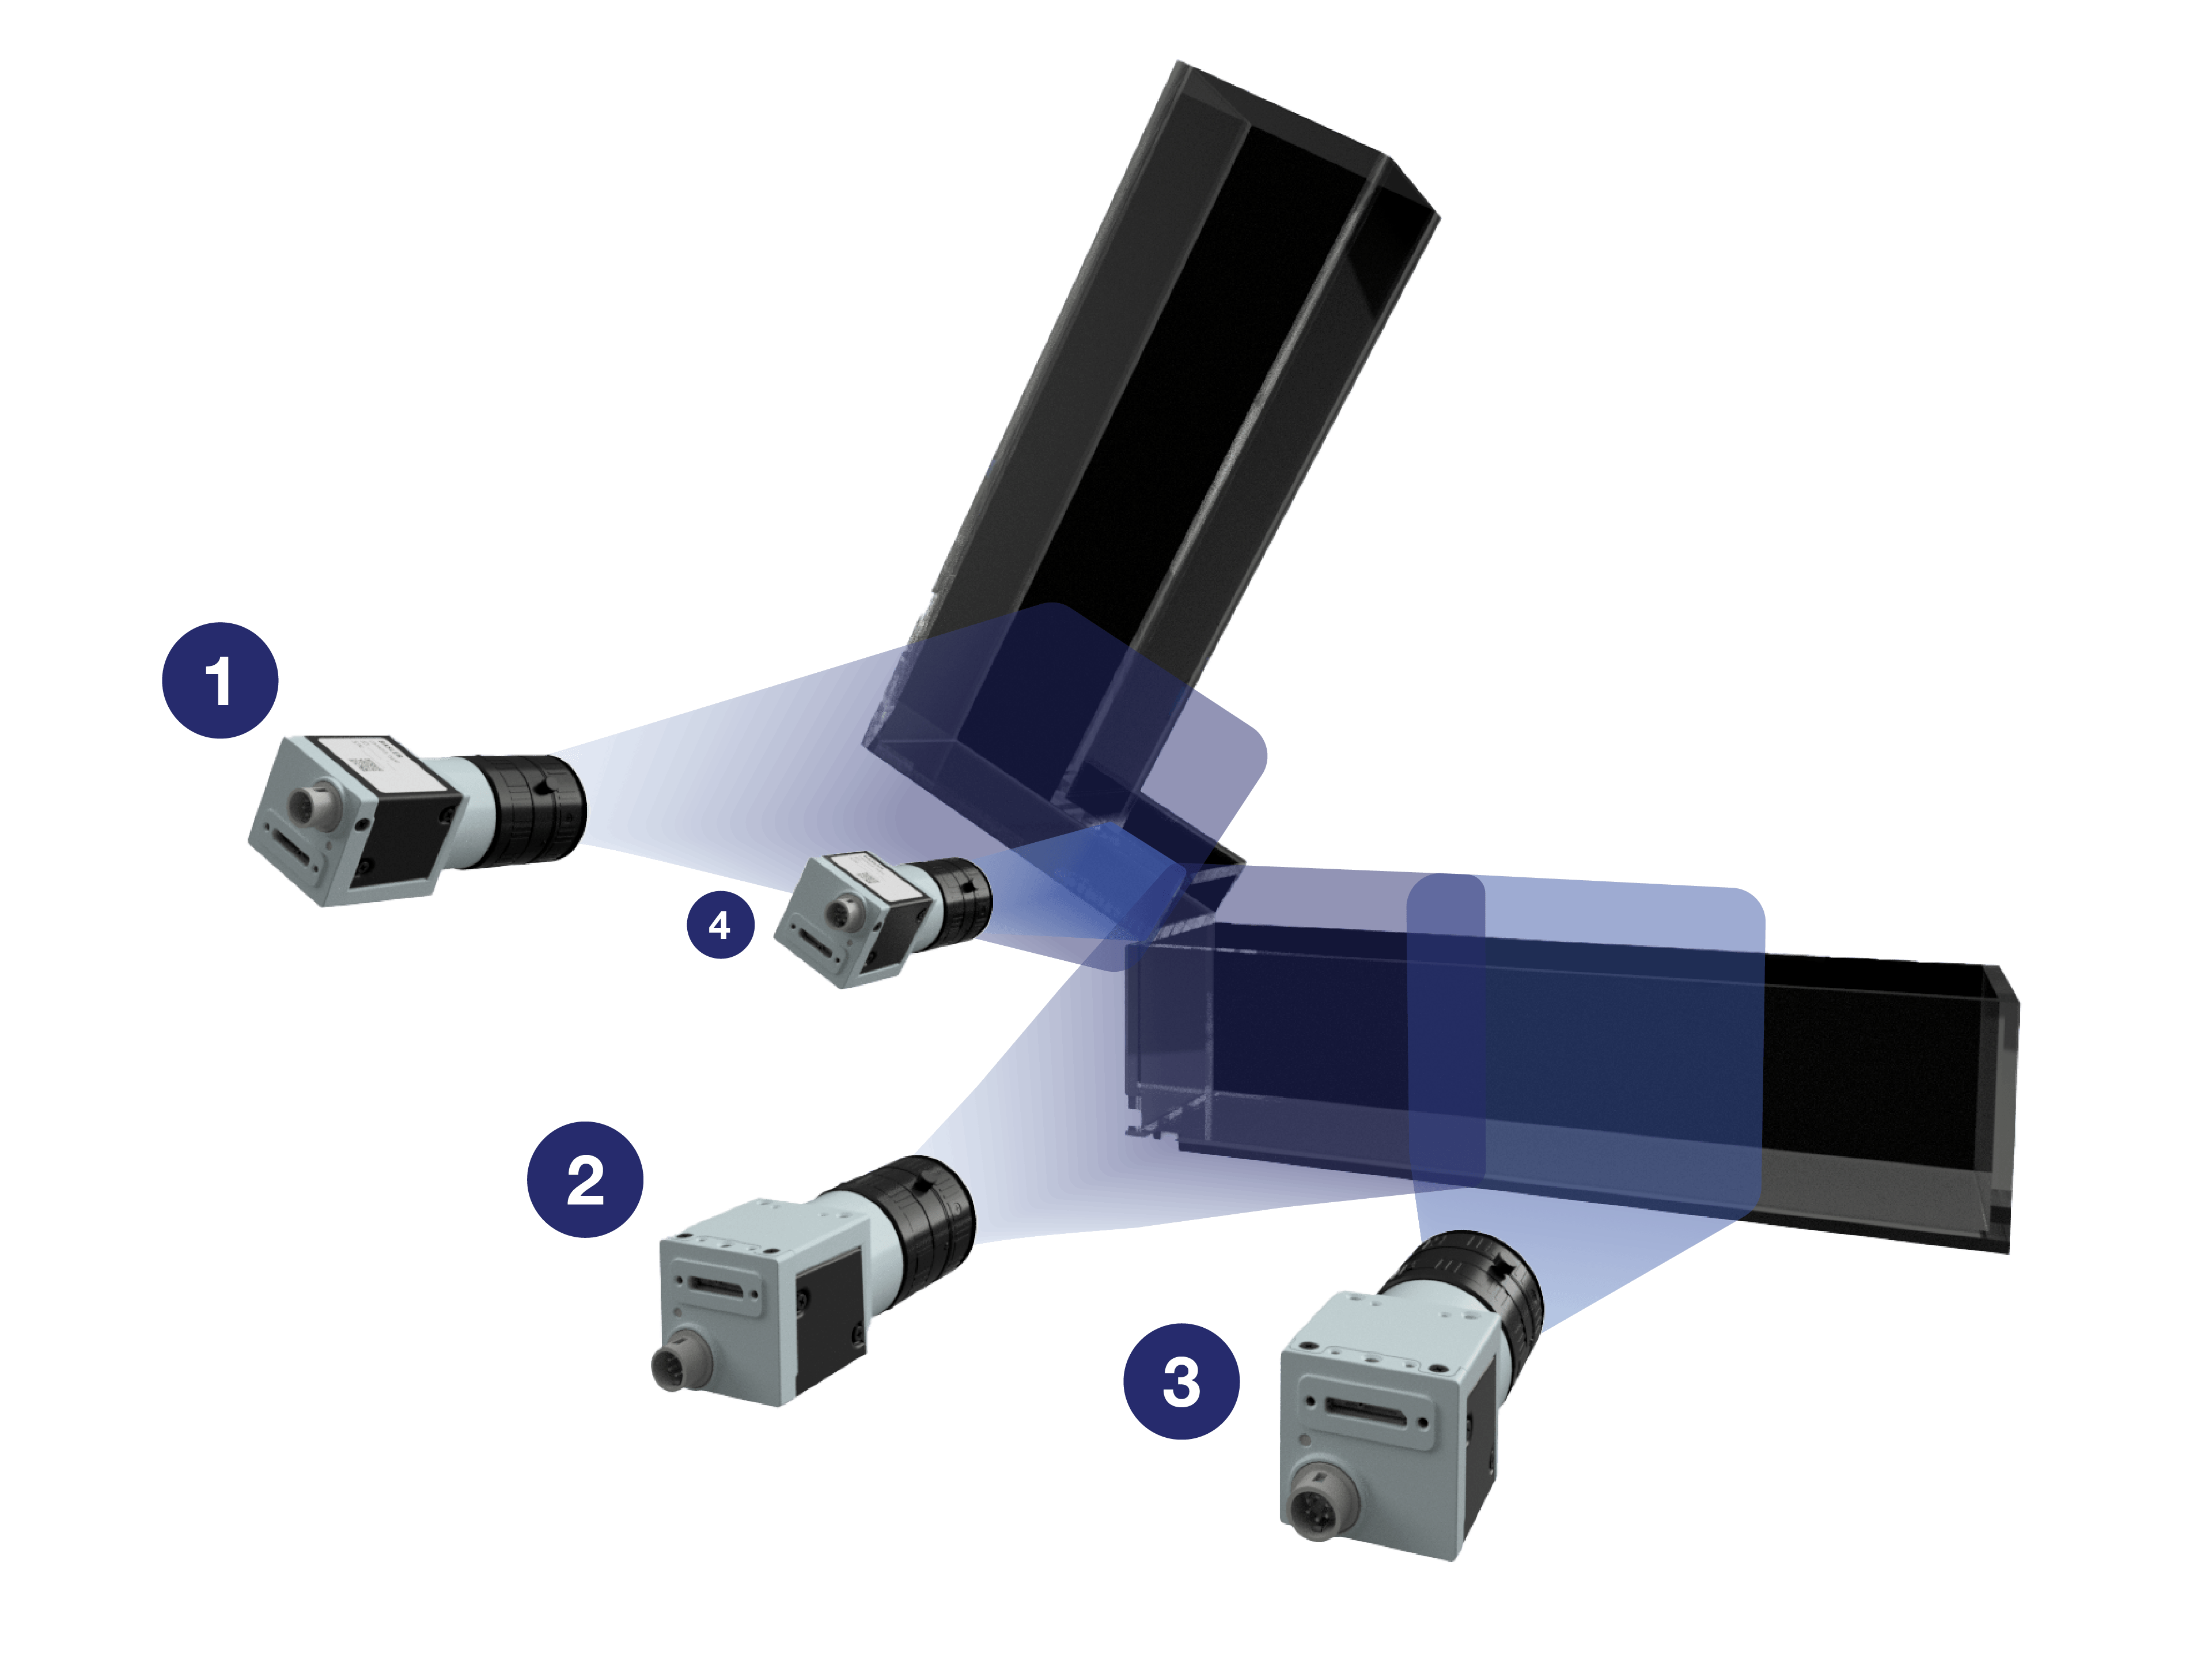
\includegraphics[width=1\textwidth]{Images/SetUpSimple.png}
    \caption{Multi-camera setup for simultaneous PIV and PTV measurements. Cameras 1--3 provide wide-field coverage of the L-shape container (Cam 1) and beam container from orthogonal views (Cams 2--3). Camera 4 captures high-speed close-up footage of the L-shape outlet region to resolve initial flow development.}
    \label{cameras_distribution}
\end{figure}

Camera 1 captures the region of interest (ROI) of the L-shape container to track overall flow progression and fiber distribution, while Cameras 2 and 3 record the beam container from orthogonal angles to enable stereoscopic reconstruction of three-dimensional fiber orientations. Camera 4 was positioned to capture a close-up view of the L-shape outlet at higher frame rate, resolving the rapid fiber reorientation occurring during the transition from vertical to horizontal flow. Table~\ref{cameras_specs} summarizes the specifications of each camera.

All cameras were equipped with 24 mm $f$/1.8 lenses. The wide aperture ($f$/1.8) enables short exposure times (reducing motion blur) at the cost of reduced depth of field. However, the shallow depth of field is acceptable because the planar laser sheet for PIV and the narrow measurement volume for PTV ensure that only features within the focal plane are illuminated and contribute to the measurements.

\begin{table}[htb]
\centering
\caption{Camera specifications and operating parameters.}
\label{cameras_specs}
\begin{tabular}{
    c
    S[table-format=3.0]
    c
    S[table-format=1.4]
}
\toprule
\textbf{Camera} & {\textbf{Frame Rate}} & \textbf{Resolution} & {\textbf{Scale Factor}} \\
 & {\textbf{(fps)}} & \textbf{(pixels)} & {\textbf{(mm/px)}} \\
\midrule
1 & 220 & 1024 $\times$ 1024 & 0.1250 \\
2 & 220 & 1024 $\times$ 1024 & 0.1282 \\
3 & 220 & 1024 $\times$ 1024 & 0.1282 \\
4 & 660 & 384  $\times$ 384  & 0.0935 \\
\bottomrule
\end{tabular}
\end{table}

\subsubsection{Illumination for PIV and PTV}

\textcolor{red}{HABLAR DE LOS TIPOS DE ILUMINACION USADAS PARA PIV Y PTV, Y JUSTIFICAR LA ELECCION DE CADA UNA.}

\begin{figure}[htb]
    \centering
    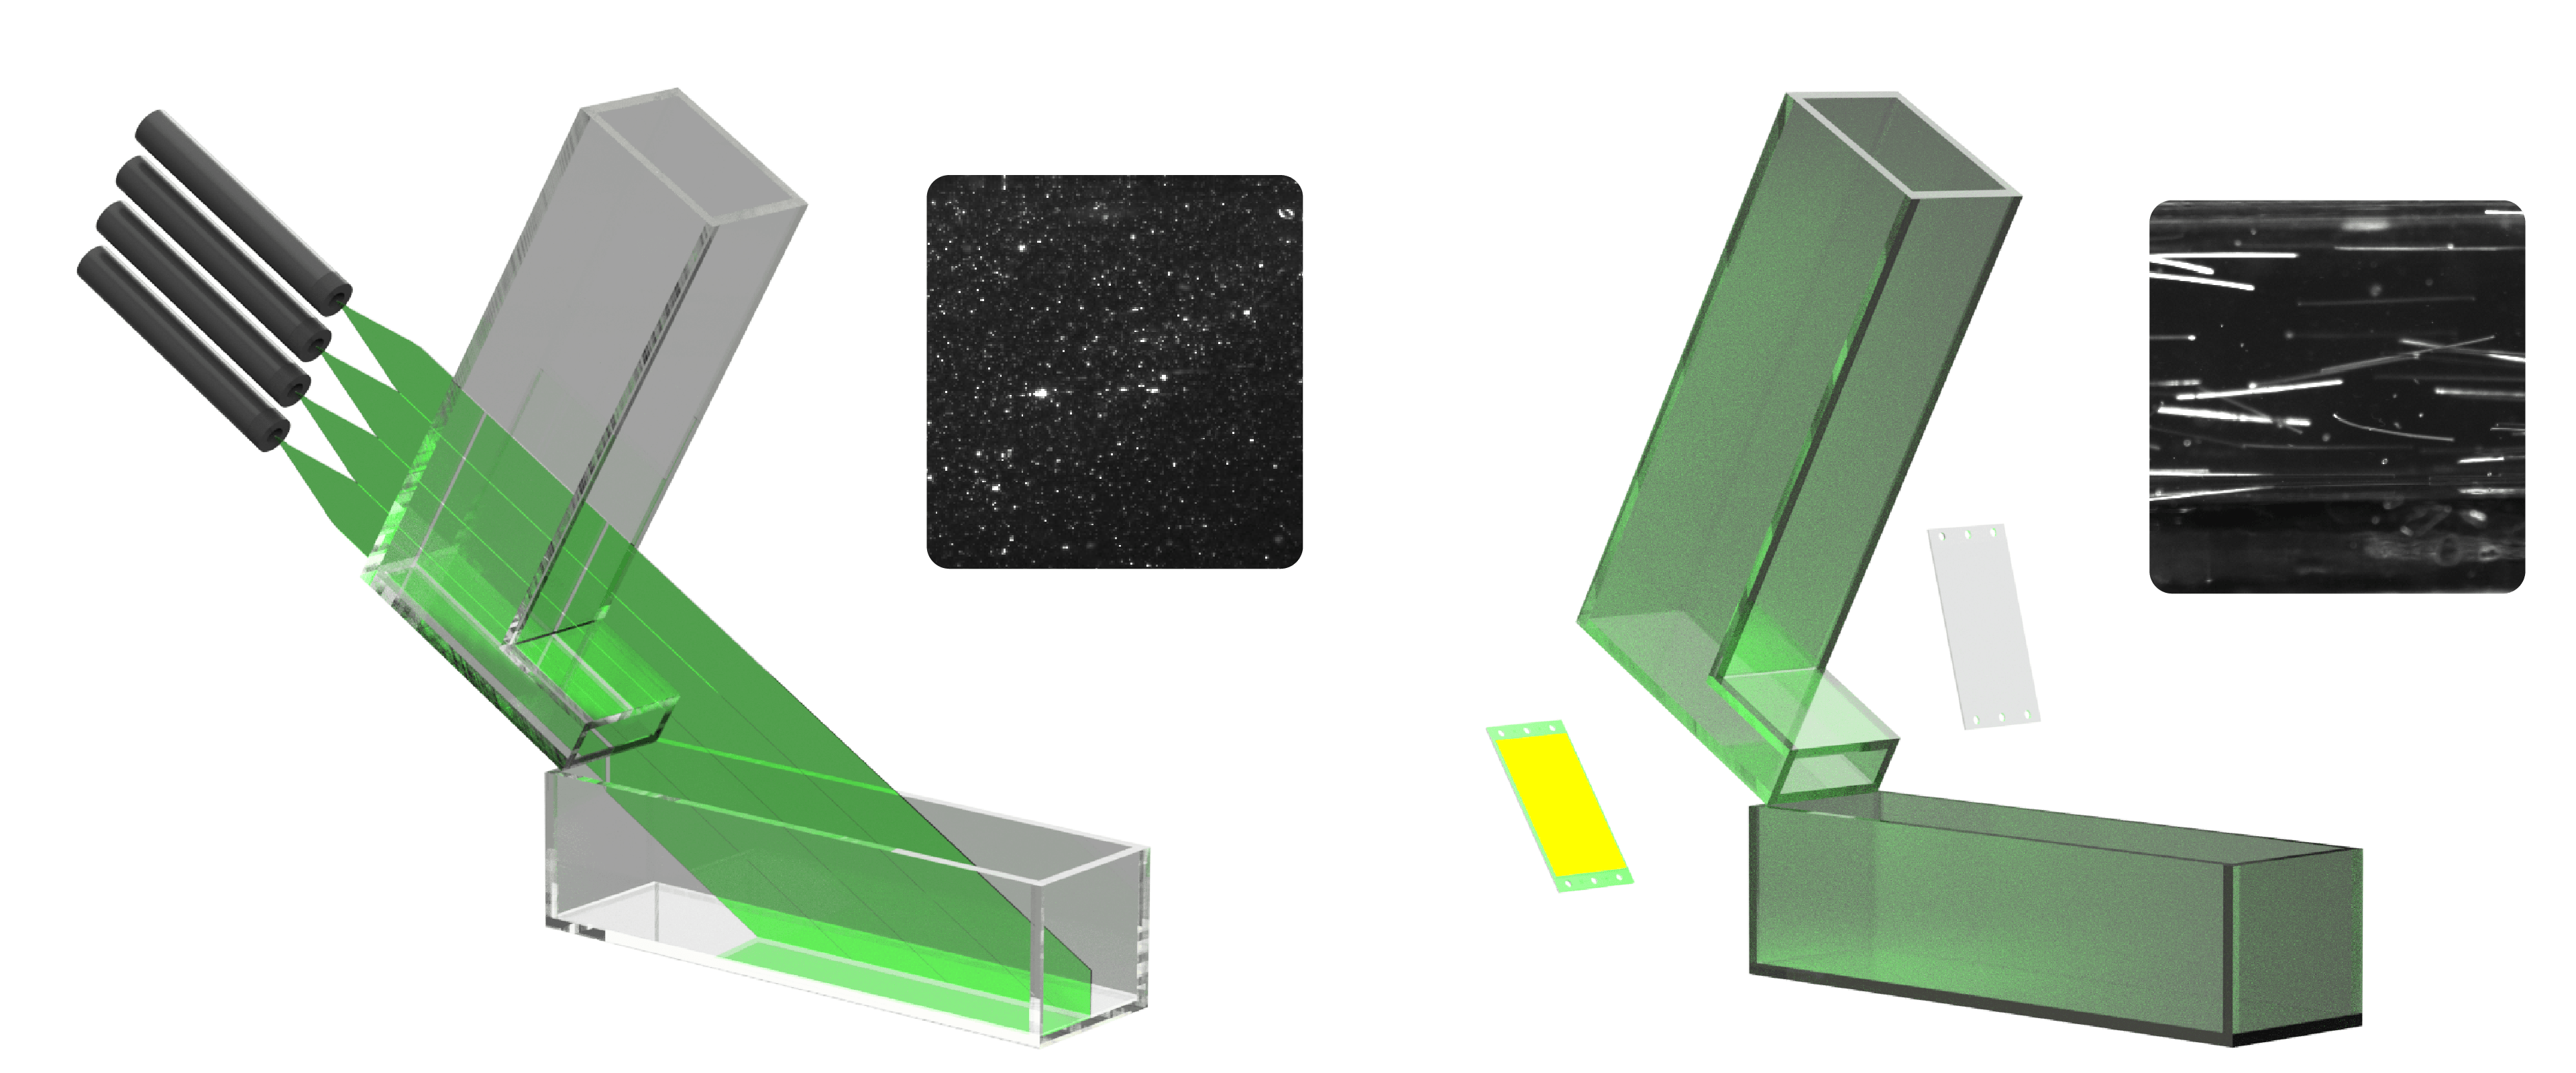
\includegraphics[width=1\textwidth]{Images/PIV and PTV basic}
    \caption{\textcolor{red}{COMPLETAR}}
    \label{cameras_distribution}
\end{figure}

\bibliographystyle{unsrt}
\bibliography{references}

\subsubsection{Experimental procedure}

The semi-dilute concentration limit was used as the primary reference for defining the fiber concentrations. For each carbopol batch prepared (2 L total volume), a volume loss of 198 $\text{mm}^3$ per fiber was estimated, yielding a final suspension volume of 1.802 L. At this volume, the semi-dilute limit of 0.024\% volume fraction corresponds to approximately 1023 fibers in the carbopol batch. Since the L-shaped device was filled only up to a height of 22.4 mm, this translates to approximately 746 fibers effectively deposited within the measurement domain. Based on this calculation, one fiber concentration below the semi-dilute limit and two above it were selected, as summarized in Table~\ref{tab:fiber_concentrations}.

Fibers were counted by weighing them on a precision balance whose resolution was at least one order of magnitude smaller than the weight of a single fiber, ensuring reliable individual fiber counts. The resulting concentrations, expressed in terms of number of fibers, weight fraction, and volume fraction, are summarized in Table~\ref{tab:fiber_concentrations}.

\begin{table}[htb]
\centering
\caption{Fiber concentrations and corresponding measurement configurations used for CFD-DEM validation. The number of fibers in $L$ refers to those deposited within the L-shaped device at a fill height of 22.4 mm.}
\label{tab:fiber_concentrations}
\begin{tabular}{
    S[table-format=5.0]
    S[table-format=2.3]
    S[table-format=1.3]
    S[table-format=5.0]
    l
}
\toprule
% Usamos \makecell para indicar dónde queremos el salto de línea con \\
{\textbf{\makecell{N° of \\ Fibers}}} &
{\textbf{\makecell{Weight \\ Fraction}}} &
{\textbf{\makecell{Volume \\ Fraction}}} &
{\textbf{\makecell{N° of Fibers \\ in $L$}}} &
{\textbf{Method}} \\
\midrule
   0 & 0.000\% & 0.000\% &    0 & PIV only \\
 750 & 0.135\% & 0.017\% &  547 & PIV \& PTV \\
1023 & 0.185\% & 0.024\% &  746 & Semi-dilute \\
1500 & 0.271\% & 0.035\% & 1094 & PIV \& PTV \\
3000 & 0.541\% & 0.069\% & 2188 & PIV \& PTV \\
\bottomrule
\end{tabular}
\end{table}

Each concentration was tested using two carbopol formulations (0.2\% and 0.5\%), to assess the sensitivity of the results to batch-to-batch rheological variability. For each formulation-concentration combination, two independent batches were prepared, and each batch was used for two experimental runs, yielding a total of 16 runs per carbopol type. In experiments with fibers, PTV was performed first to record fiber dynamics, then, tracer particles were added to the same batch to perform PIV and characterize the velocity field under identical flow conditions. In fiber-free experiments, two PIV runs were performed per batch. Across all test per formulation, this protocol resulted in 10 PIV datasets and 6 PTV datasets per formulation.

Figure~\ref{fig:validationtest} shows representative images of the L-shaped device prior to each experimental run, illustrating the progressive increase in fiber density across the tested concentrations. These images confirm the visual distinction between loading conditions and provide qualitative context for the quantitative tracking results discussed in Section~\ref{sec:ptv_validation_results}.

\begin{figure}[htb]
    \centering
    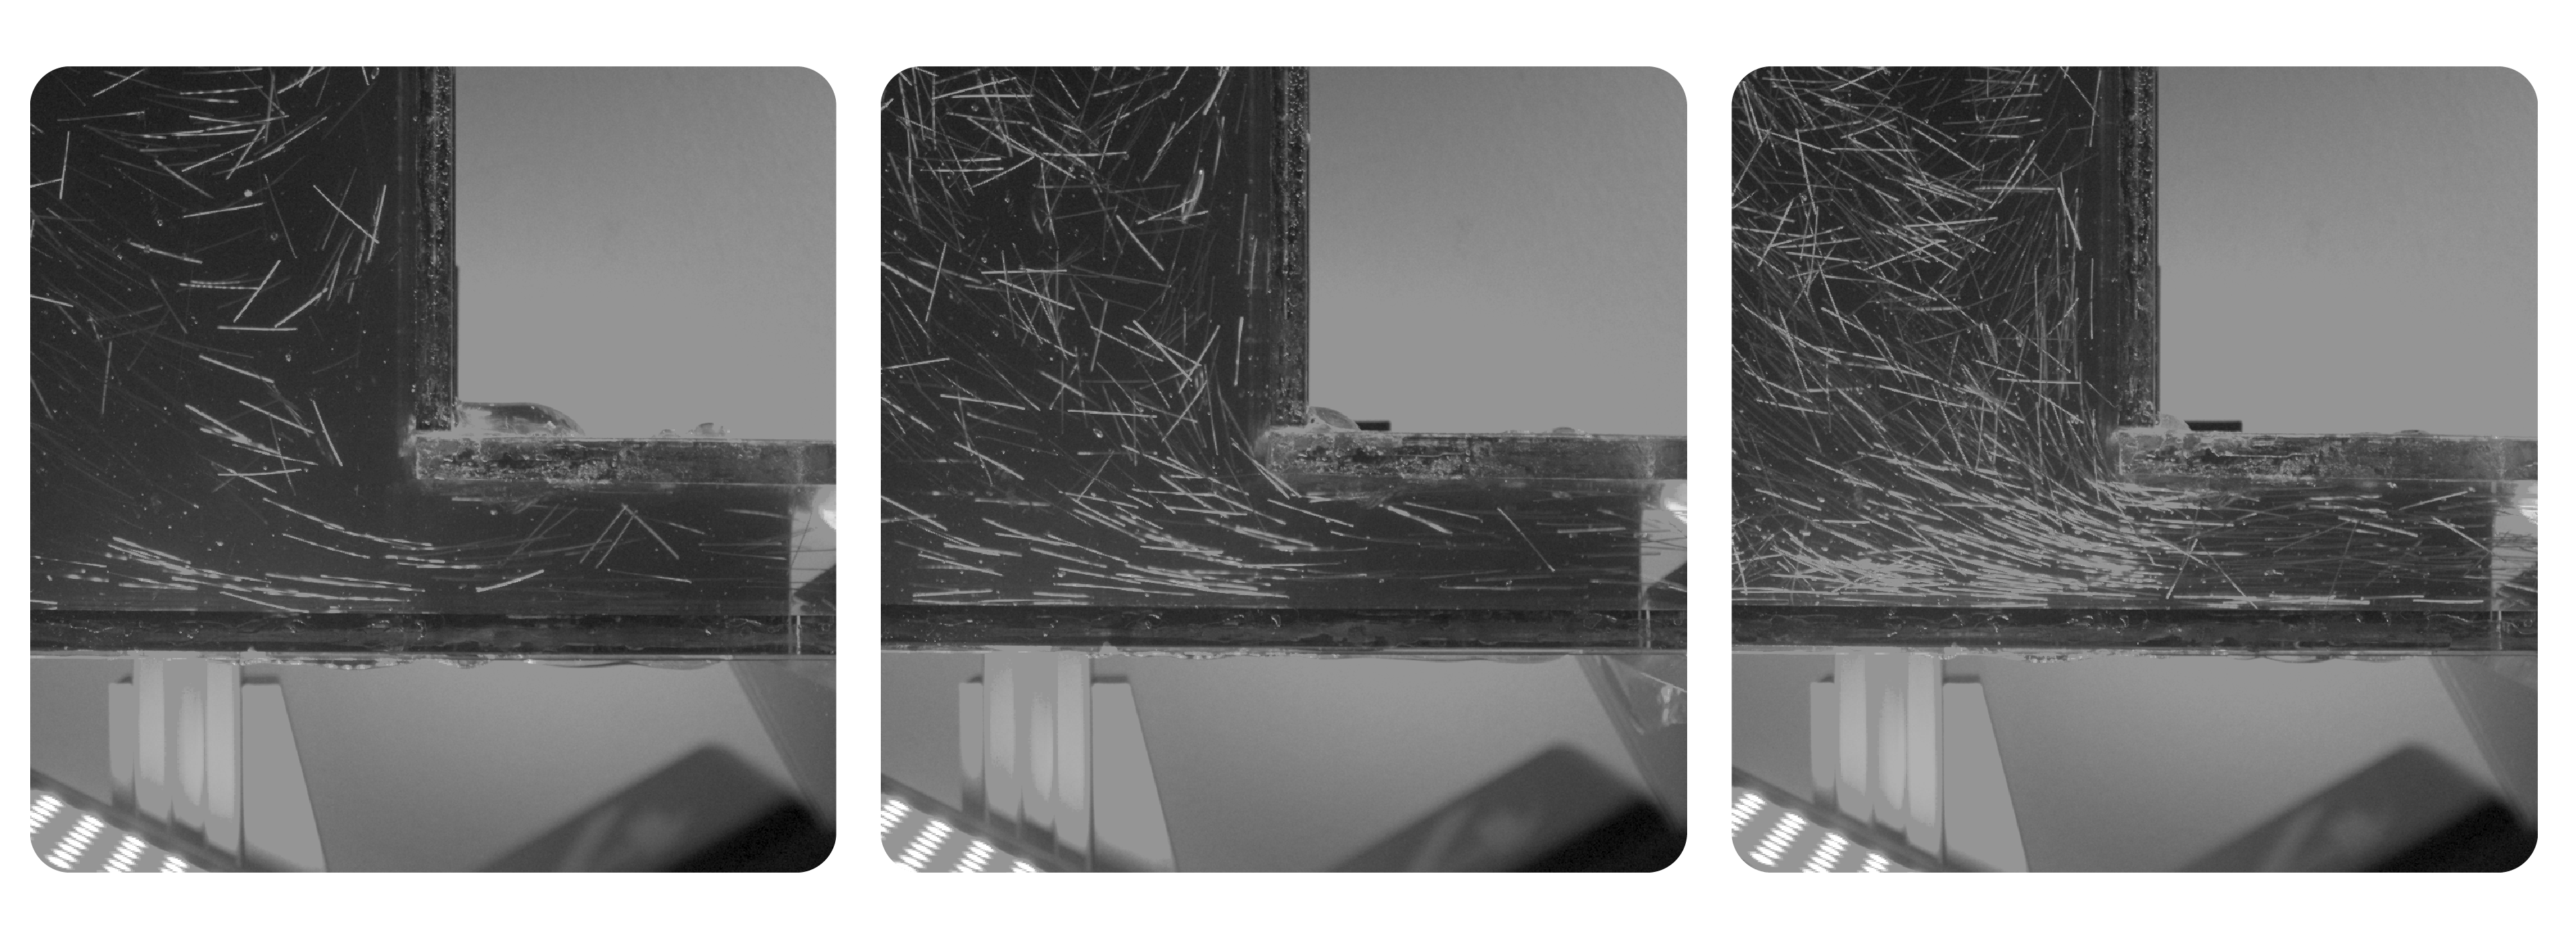
\includegraphics[width=1\textwidth]{Images/ValidationTakes.png}
    \caption{Representative images of the L-shaped device prior to experimental runs at each fiber concentration: 750 fibers, 1500 fibers and 3000 fibers, shown for both Carbopol-02 and Carbopol-05 formulations. Images illustrate the progressive increase in fiber density and spatial overlap as fiber loading increases.}
    \label{fig:validationtest}
\end{figure}


\end{document}